\documentclass{beamer}\usepackage[]{graphicx}\usepackage[]{color}
%% maxwidth is the original width if it is less than linewidth
%% otherwise use linewidth (to make sure the graphics do not exceed the margin)
\makeatletter
\def\maxwidth{ %
  \ifdim\Gin@nat@width>\linewidth
    \linewidth
  \else
    \Gin@nat@width
  \fi
}
\makeatother

\definecolor{fgcolor}{rgb}{0.345, 0.345, 0.345}
\newcommand{\hlnum}[1]{\textcolor[rgb]{0.686,0.059,0.569}{#1}}%
\newcommand{\hlstr}[1]{\textcolor[rgb]{0.192,0.494,0.8}{#1}}%
\newcommand{\hlcom}[1]{\textcolor[rgb]{0.678,0.584,0.686}{\textit{#1}}}%
\newcommand{\hlopt}[1]{\textcolor[rgb]{0,0,0}{#1}}%
\newcommand{\hlstd}[1]{\textcolor[rgb]{0.345,0.345,0.345}{#1}}%
\newcommand{\hlkwa}[1]{\textcolor[rgb]{0.161,0.373,0.58}{\textbf{#1}}}%
\newcommand{\hlkwb}[1]{\textcolor[rgb]{0.69,0.353,0.396}{#1}}%
\newcommand{\hlkwc}[1]{\textcolor[rgb]{0.333,0.667,0.333}{#1}}%
\newcommand{\hlkwd}[1]{\textcolor[rgb]{0.737,0.353,0.396}{\textbf{#1}}}%
\let\hlipl\hlkwb

\usepackage{framed}
\makeatletter
\newenvironment{kframe}{%
 \def\at@end@of@kframe{}%
 \ifinner\ifhmode%
  \def\at@end@of@kframe{\end{minipage}}%
  \begin{minipage}{\columnwidth}%
 \fi\fi%
 \def\FrameCommand##1{\hskip\@totalleftmargin \hskip-\fboxsep
 \colorbox{shadecolor}{##1}\hskip-\fboxsep
     % There is no \\@totalrightmargin, so:
     \hskip-\linewidth \hskip-\@totalleftmargin \hskip\columnwidth}%
 \MakeFramed {\advance\hsize-\width
   \@totalleftmargin\z@ \linewidth\hsize
   \@setminipage}}%
 {\par\unskip\endMakeFramed%
 \at@end@of@kframe}
\makeatother

\definecolor{shadecolor}{rgb}{.97, .97, .97}
\definecolor{messagecolor}{rgb}{0, 0, 0}
\definecolor{warningcolor}{rgb}{1, 0, 1}
\definecolor{errorcolor}{rgb}{1, 0, 0}
\newenvironment{knitrout}{}{} % an empty environment to be redefined in TeX

\usepackage{alltt}
\mode<presentation> {

% The Beamer class comes with a number of default slide themes
% which change the colors and layouts of slides. Below this is a list
% of all the themes, uncomment each in turn to see what they look like.

%\usetheme{default}
%\usetheme{AnnArbor}
%\usetheme{Antibes}
%\usetheme{Bergen}
%\usetheme{Berkeley}
%\usetheme{Berlin}
%\usetheme{Boadilla} %like
%\usetheme{CambridgeUS}
%\usetheme{Copenhagen}
%\usetheme{Darmstadt}
%\usetheme{Dresden}
%\usetheme{Frankfurt}
%\usetheme{Goettingen} %like
\usetheme{Hannover} %like
%\usetheme{Ilmenau}
%\usetheme{JuanLesPins}
%\usetheme{Luebeck}
%\usetheme{Madrid}
%\usetheme{Malmoe}
%\usetheme{Marburg}
%\usetheme{Montpellier}
%\usetheme{PaloAlto}
%\usetheme{Pittsburgh}
%\usetheme{Rochester}
%\usetheme{Singapore}
%\usetheme{Szeged}
%\usetheme{Warsaw}

% As well as themes, the Beamer class has a number of color themes
% for any slide theme. Uncomment each of these in turn to see how it
% changes the colors of your current slide theme.

%\usecolortheme{albatross}
%\usecolortheme{beaver}
%\usecolortheme{beetle}
%\usecolortheme{crane}
%\usecolortheme{dolphin}
%\usecolortheme{dove}
%\usecolortheme{fly}
%\usecolortheme{lily}
%\usecolortheme{orchid}
%\usecolortheme{rose}
%\usecolortheme{seagull}
%\usecolortheme{seahorse}
%\usecolortheme{whale}
%\usecolortheme{wolverine}

%\setbeamertemplate{footline} % To remove the footer line in all slides uncomment this line
%\setbeamertemplate{footline}[page number] % To replace the footer line in all slides with a simple slide count uncomment this line

%\setbeamertemplate{navigation symbols}{} % To remove the navigation symbols from the bottom of all slides uncomment this line
}

\usepackage{graphicx} % Allows including images
\usepackage{booktabs} % Allows the use of \toprule, \midrule and \bottomrule in tables
\usepackage{pgfpages}
\usepackage{amsmath}


%----------------------------------------------------------------------------------------
%	TITLE PAGE
%----------------------------------------------------------------------------------------

\title[Computation \& optimization]{Computation \& optimization for Lasso - part 2} % The short title appears at the bottom of every slide, the full title is only on the title page

\author{Luyang Han \& Janosch Ott} % Your name
\institute[] % Your institution as it will appear on the bottom of every slide, may be shorthand to save space
{
ETH Zurich \\ % Your institution for the title page
%\medskip
%\textit{john@smith.com} % Your email address
}
\date{22 October 2018} % Date, can be changed to a custom date

\setbeamercovered{transparent} % else hidden elements are gray, this way they are invisible
\setbeamertemplate{navigation symbols}{} %comment to have a lot of navigating symbols
\setbeamertemplate{section in toc}[sections numbered] % removes the ugly balls
%\setbeameroption{show notes}
\setbeameroption{show notes on second screen=right}
\setbeamertemplate{enumerate items}[default] % to get rid of some more ugly balls


%%%%%%%% ------------%%%%%%%%%%-----------%%%%%%%%%%%------------%%%%%%%%%%-----------
\newcommand{\R}{\mathbb{R}}
\newcommand{\Norm}[1]{\left\lVert#1\right\rVert}
\newcommand{\norm}[1]{\left\lvert#1\right\rvert}
\DeclareMathOperator*{\argmin}{arg\,min}
\DeclareMathOperator*{\argmax}{arg\,max}



%%%%%%%%%%% ----------%%%%%%%%%%-----------%%%%%%%%%%------------%%%%%%%%%--------------


\usepackage{hyperref}
\IfFileExists{upquote.sty}{\usepackage{upquote}}{}
\begin{document}



% very important to use option [fragile] for frames containing code output!
  
  \begin{frame}[fragile]
You can test if \textbf{knitr} works with this minimal demo. OK, let's
get started with some boring random numbers:

\begin{knitrout}\footnotesize
\definecolor{shadecolor}{rgb}{0.969, 0.969, 0.969}\color{fgcolor}\begin{kframe}
\begin{alltt}
\hlkwd{set.seed}\hlstd{(}\hlnum{1121}\hlstd{)}
\hlstd{(x}\hlkwb{=}\hlkwd{rnorm}\hlstd{(}\hlnum{20}\hlstd{))}
\end{alltt}
\begin{verbatim}
##  [1]  0.1449583  0.4383221  0.1531912  1.0849426  1.9995449 -0.8118832
##  [7]  0.1602680  0.5858923  0.3600880 -0.0253084  0.1508809  0.1100824
## [13]  1.3596812 -0.3269946 -0.7163819  1.8097690  0.5084011 -0.5274603
## [19]  0.1327188 -0.1559430
\end{verbatim}
\begin{alltt}
\hlkwd{mean}\hlstd{(x);}\hlkwd{var}\hlstd{(x)}
\end{alltt}
\begin{verbatim}
## [1] 0.3217385
## [1] 0.5714534
\end{verbatim}
\begin{alltt}
\hlcom{# n = 100}
\hlcom{# par(mfrow=c(1,3))}
\hlcom{# r = 0.1}
\hlcom{# x1 = rnorm(n)}
\hlcom{# x2 = rnorm(n)}
\hlcom{# y1 = r*x2+sqrt(1-r*r)*x1}
\hlcom{# plot(y1,x2, main = "rho = 0.1", xlab = "x_j", ylab = "y")}
\hlcom{# r = 0.5}
\hlcom{# x1 = rnorm(n)}
\hlcom{# x2 = rnorm(n)}
\hlcom{# y1 = r*x2+sqrt(1-r*r)*x1}
\hlcom{# plot(y1,x2, main = "rho = 0.5", xlab = "x_j", ylab = "y")}
\hlcom{# r = 0.9}
\hlcom{# x1 = rnorm(n)}
\hlcom{# x2 = rnorm(n)}
\hlcom{# y1 = r*x2+sqrt(1-r*r)*x1}
\hlcom{# plot(y1,x2, main = "rho = 0.9", xlab = "x_j", ylab = "y")}
\end{alltt}
\end{kframe}
\end{knitrout}
\end{frame}

\begin{frame}[fragile]
The first element of \texttt{x} is 0.1449583. Boring boxplots
and histograms recorded by the PDF device:

\begin{knitrout}\footnotesize
\definecolor{shadecolor}{rgb}{0.969, 0.969, 0.969}\color{fgcolor}
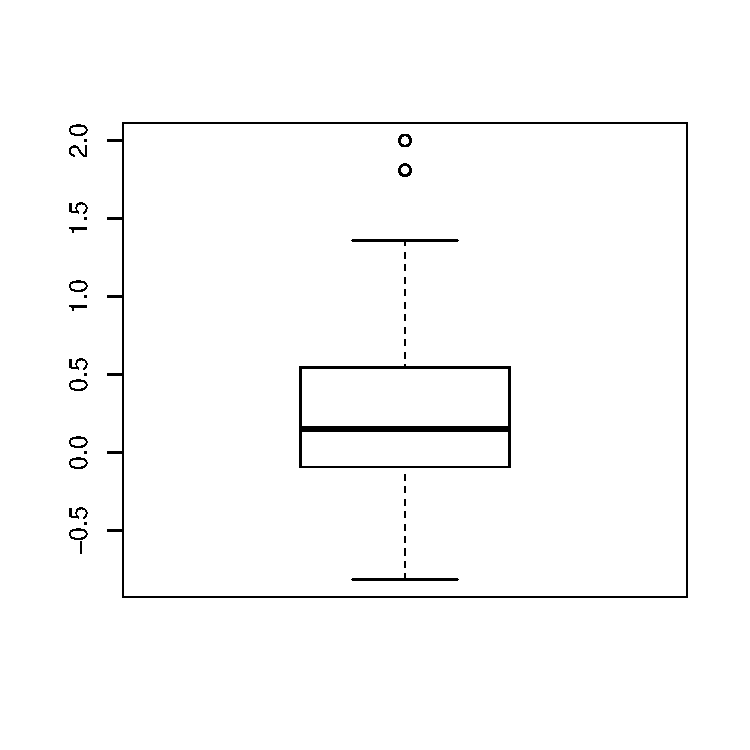
\includegraphics[width=.30\linewidth]{figure/boring-plots-1} 
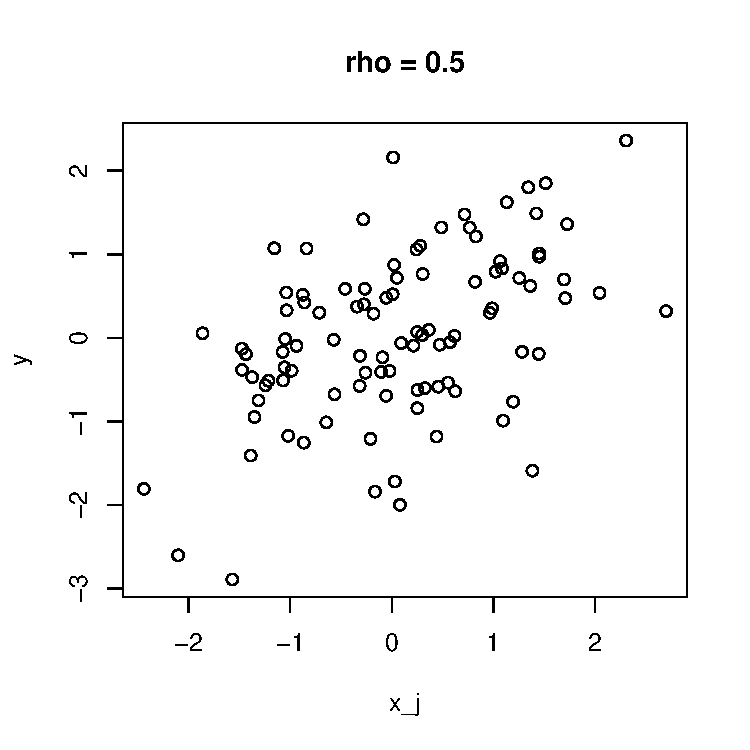
\includegraphics[width=.30\linewidth]{figure/boring-plots-2} 
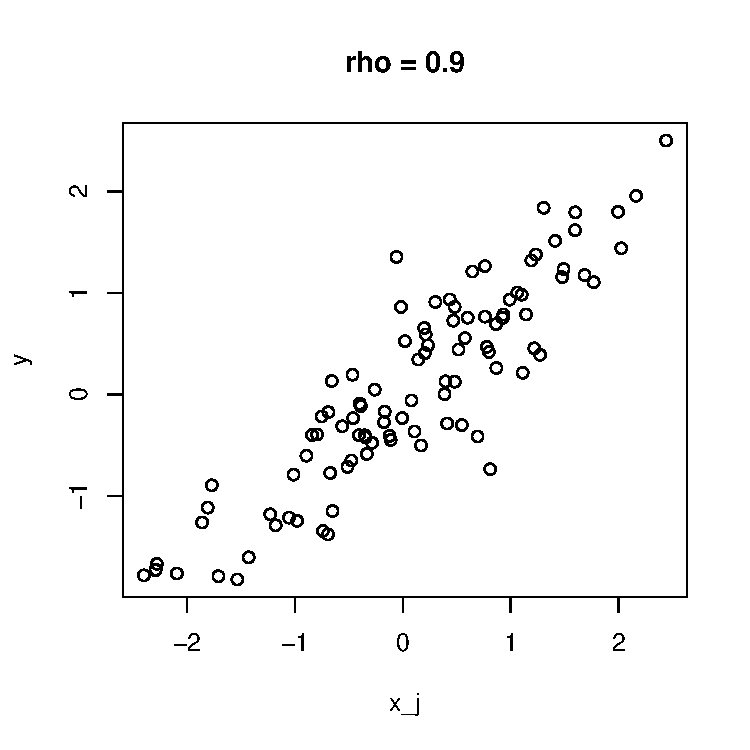
\includegraphics[width=.30\linewidth]{figure/boring-plots-3} 

\end{knitrout}
\end{frame}

\end{document}
